\fancychapter{Optimization System}
\label{sec:os_implementation}


This chapter introduces the considered optimization algorithms to produce a solution to a Flying Tourist Problem, as defined in section \ref{sec:ftp}. 
Given the real-world application under development, and its goals, the devised optimization system should be capable of providing a stream of responses in finite-time. Due to these objectives, the considered optimization strategies are based on heuristic algorithms (section \ref{sec:heuristic}) and meta heuristics algorithms (section \ref{sec:meta}), as the characteristics of these algorithms fit the goals of the system.




\section{Initial Response}
\label{sec:initial_response}

\todo{Do not start like this. INitial responnse?! We have to definew what we want. We have to define how to get it. And we have to see the advantages and disadvantages of each of the porposed solutions. Also, we want to define what is important. From the user pov. We also need to explain how this affects our choices. This chapter structure should be. 1) Goals, 2) How 3) Why}

\todo{Insert heuristics like NN, two opt, random too.}

\todo{If possible, find out the polynomial time of each of the constructed algorithms.}
Consider a user request which defines a start period $T_0=[T_{0i}, T_{0f}]$,
a start city, $v_0$, a return city $v_{n+1}$, and a list of cities to be visited,
$V$, where upon visiting each city $i$ $\in$ $V$, a waiting periof of $d_i$ days is necessary.

The steps necessary to construct a random solution to this request are illustrated in figure \ref{fig:random_solution},
and can be summarized as follows. Start by setting the initial time, $t \in T_0$, and the current node, $v_c = v_0$.
If there are no nodes to visit, that is, if $V = \{\}$, a solution if defined by the flight $a_{v_0, v_{n+1}}^{t}$.
Otherwise, select a random city, $v_i \in V$,
and extend the solution with the flight $a_{v_c, v_{i}}^{t}$. Follow this with the update of $t = t + d_i$,
remove the selected node $v_i$ from $V$, and set it as the current node.
Repeat this process untill all nodes are visited, and conclude by closing the tour.

The described process may start immediatly after receiving a request,
because it does not require the information relative to the arcs of the problem.
Instead, it generates a completly random solution, composed of several flights,
whose information is not yet known. 
Thus, this solution is passed to the Data Management System, which calls a third-party API 
to request the relevant information. If the number of flights which constitute the solution is lower than 9,
this information can be obtained with a single HTTP request to the API. Otherwise, the number of necessary requests 
is given by, approximately, $N/10 + 1$, where $N$ is the number of necessary flights.


% \begin{enumerate}
%   \item set an initial empty solution, $s$ = ();
%   \item select a start date, $t_0 \in T_0$;
%   \item define the current node $v_c = v_0$, and the current time $t = t_0$;
%   \item if V = $\{\}$ go to step 9);
%   \item select a random city $v_i \in V$;
%   \item extend the solution $s$ with the arc $a_{v_c, v_i}^{t}$;
%   \item increment time: $t = t + d_i$, and set current node $v_a = v_i$, remove $v_i$ from $V$;
%   \item go to step 4);
%   \item extend the solution $s$ with the arc $a_{v_c, v_{n+1}}^{t}$;
% \end{enumerate}

\begin{figure}[htpb]
  \centering
  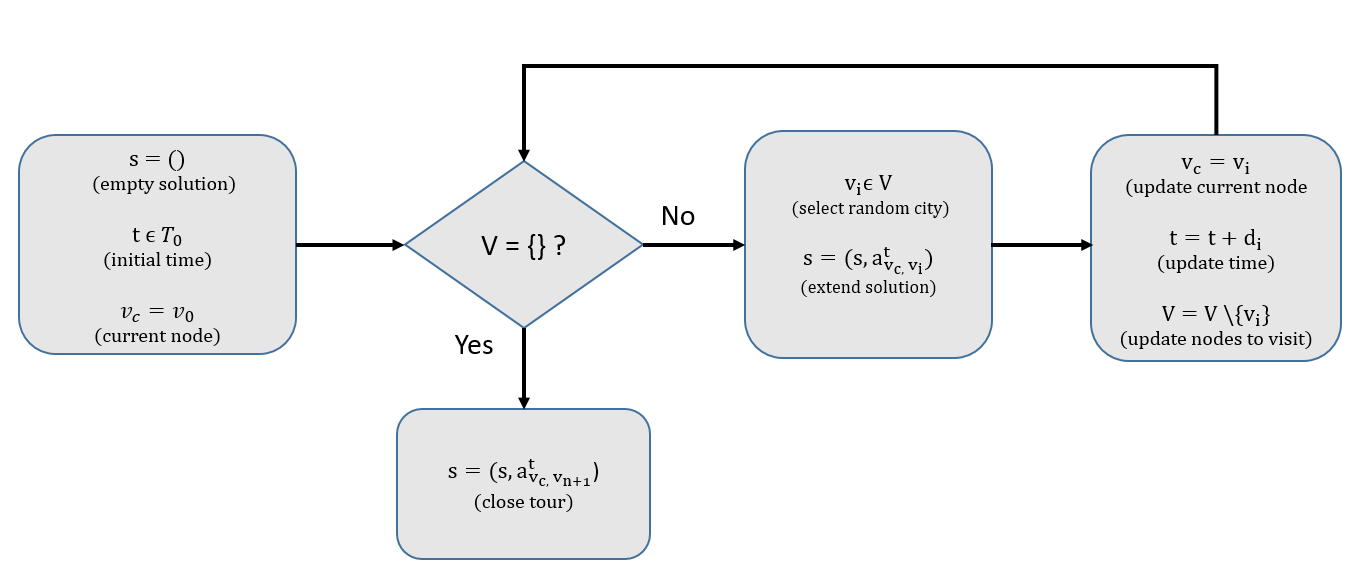
\includegraphics[width=\textwidth]{Figures/system_implementation/random_solution.png}
  \caption{Steps to generate a random solution to a user request.}
  \label{fig:random_solution}  
\end{figure}

While the random solution generation may start immediatly after receiving a request,
the nearest neighbour heuristic relies on a complete cost matrix,
and so can not be initiated before collecting all the information necessary.
The nearest neighbour algorithm is closely related to the process described in figure \ref{fig:random_solution},
however, instead of selecting a random node $i \in V$,
this node is selected according to its cost. At any point of the process, there is a \textit{current} node and time,
which can be used to determine all the possible solution components (arcs), where the one with the lowest cost is selected.
Furthermore, if the start time of the request is given by a time window,
the illustrated process can be repeated for all allowable start dates.








\section{Ant Colony Optimization}
\label{sec:aco_implementation}
Figure \ref{fig:aco_block_diagram} presents a block diagram illustrating the Ant
Colony Optimization metaheuristic. The algorithm receives a weight matrix which
contains the information relative to the arcs of the bipartite graph describing
the problem, aswell as other relevant data, as the duration set $D$, associated
to each city $i$, of the set of nodes to be visited, $V$. After the
initialisation, and untill the termination condition is met, the algorithm
performs a cycle, in which every agent constructs a solution to the problem,
followed by a pherormone matrix update, to reflect the search experience of each
ant.

\begin{figure}[htpb]
  \centering
  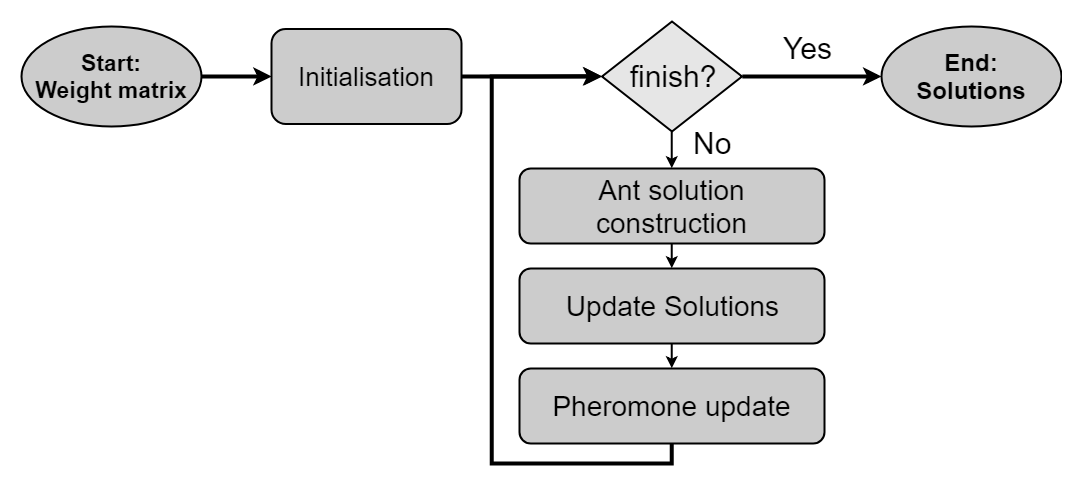
\includegraphics[width=\textwidth]{Figures/system_implementation/aco_base.png}
  \caption{Block diagram of the Any Colony Optimization metaheuristic.}
  \label{fig:aco_block_diagram}  
\end{figure}

The initialisation of the ACO metaheuristic requires the construction of an
initial pherormone matrix. As suggested by the ACO authors \cite{aco_2}, the
value of each entry of the pherormone matrix is given by equation
\ref{eq:pheromone_init}, which is inversely proportional to the cost of the
nearest neighbour solution, $C^{nn}$. The initialisation of the metaheuristic
also requires the definition of a variety of algorithm specific parameters, as
the number of ants $m$, the pherormone evaporation rate $\rho$, the heuristic
relative influence $\beta$, the pherormone relative influence $\alpha$, and the
exploration rate $Q_0$. 

\begin{equation}
\label{eq:pheromone_init}
  \tau_{ij}^{t} = \tau_{0} = \frac{1}{nC^{nn}}
\end{equation}

The construction process undertaken by each ant, illustrated in figure
\ref{fig:aco_construction} is as follows. First, the current time is set to a
value belonging to the allowable start dates, $t \in T_0$, and the current node
is set to the start node $v_0$. Each ant enters than an iterative cycle untill
all nodes belonging to $V$ are visited. At every step of this cycle, an ant
chooses a solution component by either \textit{exploiting} or \textit{exploring}
the search space. The decision of exploiting or exploring depends on the
algorithm parameter $Q_0$, and a pseudo-random value $q$, calculated at run
time. The selection of the solution component $j$, which identifies the next
city to be visited, is thus given by equation \ref{eq:selection_rule}. After the
selection of each solution component, it is necessary to update the time,
incrementing it by the duration relative to the selected city.

\begin{figure}[htpb]
  \centering
  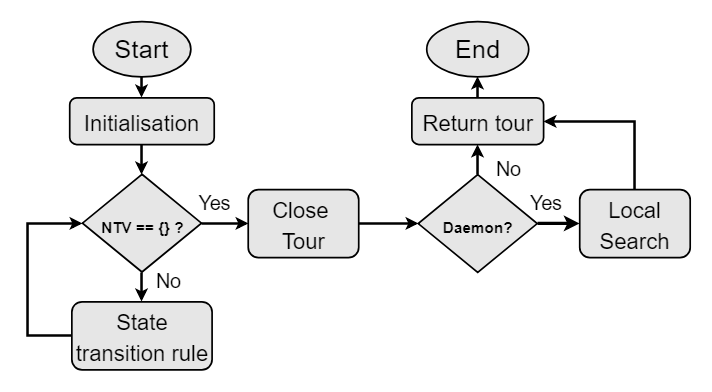
\includegraphics[width=\textwidth]{./Figures/system_implementation/aco_construction.png}
  \caption{Block diagram of the construction procedure undertaken by each ant.}
  \label{fig:aco_construction}  
\end{figure}

\begin{equation}
  \label{eq:selection_rule}
  j =  \left \{
    \begin{aligned}
      & exploitation \ (\text{eq.} \ \ref{eq:exploitation}) , && \text{if}\ q \leq Q_0 \\
      & exploration \ (\text{eq.} \ \ref{eq:exploration}), && \text{otherwise}
    \end{aligned} \right. 
\end{equation}

The exploration of the search space utilizes the so called
\textit{random-proportional rule}, given by equation \ref{eq:exploitation},
which determines the next solution component of the ants solution. Note that
$J_k(i,t)$ is the set of the solutions components which might be selected and
form a valid solution, by an ant which is currently at city $i$ at time $t$. In
its turn, the exploration is given by equation \ref{eq:exploration}, and
$p_a(i,j,t)$ represents the probability of ant $a$, which is currently at the
node $i$ at time $t$, selecting $j$ as the next node to visit. In the presented
equations, $\eta$ is the inverse of the weight matrix value.

\begin{equation}
  \label{eq:exploitation}
    arg max_{j \in J_k(i,t)} {[\tau(i,j,t)][\eta(i,j,t)]^\beta}
\end{equation}


\begin{equation}
\label{eq:exploration}
  p_a(i,j,t) =  \left \{
    \begin{aligned}
      & \frac{[\tau(i,j,t)][\eta(i,j,t)]^\beta}{\sum_{u \in J_k(i,t)}[\tau(i,u,t)][\eta(i,u,t)]^\beta}, && \text{if}\ j \in J_k(i,t) \\
      &0, && \text{otherwise}
    \end{aligned} \right. 
\end{equation}

Follwing the iterative construction procedure, an uncomplete solution is
available. To complete this solution, it is necessary to add an extra solution
component, which connects the last visited node, to the return node, $v_{n+1}$.

Having a complete solution, it is possible to perform \textit{Daemon Actions},
or in other words, try to improve the constructed solution using a local search
algorithm. The execution of this step is optional, and is set by a parameter
algorithm at the initialization of the procedure. The selection of a local
search algorithm is usually problem specific, and for the Traveling Salesman
Problem, one of the most used local search procedures is the $k$-opt exchange.
During the development of this work, the 2-opt procedure was utilized.

The mainstream success of the Ant Colony Optimization in the multiple areas in
which it was applied, is due to its ability to \textit{guide} the agents to good
solutions. While the construction of each solution follows a pseudo-random rule,
the overall quality of this solution is used to bias the search towards the
search space around this solution. This achieved by the global pheromone update,
given by equation \ref{eq:global_update}.


\begin{equation}
\label{eq:global_update}
  \tau_{ijt} = (1-\rho)\tau_{ijt} + \sum_{s \in S_{upd} | c_{ijt} \in s} g(s)
\end{equation}

The global pheromone update is a proccess in which, at every step of the
algorithm, all entries of the pheromone matrix are updated, by the so called
pheromone \textit{evaporation} and \textit{depositation}. Pheromone evaporation
is a method used to avoid getting stuck in sub-optimal solutions, while
pheromone deposition intends to induce the exploration of the search space
around good solutions, by incrementing the pheromone values of the solution
components belonging to a set $S_{upd}$. The set $S_{upd}$ is usually a subset
of the solutions constructed at the current iterative step, $S_{upd} \subset
S_{iter}$. Furthermore, the set $S_{upd}$ includes the best global solution
$S_{best}$, and this work follows the elitist ant rule, which defines that
pheromone deposition on the solution components beloning to $S_{best}$ is
actually higher than those of the other solutions in $S_{upd}$. In equation
\ref{eq:global_update}, $g(): S \rightarrow \mathcal{R}^+$ is a function such
that $f(s) < f(s^{'}) \Rightarrow g(s) \geq g(s^{'})$. It is common set $g()$ to
be inversely proportional to the objective function $f()$. Thus, the inversely
proportional constant for $g$ is set to $1$ for all solution components in
$S_{upd}$, and to a higher value for $S_{best}$, 3 in this case, due to the
elitist ant rule.








\section{Simulated Annealing}
\label{sec:sa_implementation}
The Simulated Annealing is a metaheuristic for solving continuous and discrete combinatorial optimization problem,
and it is well known for its ability to escape from local minima. 
Every SA algorithm is composed of a main cycle, and a secondary cycle, which is often refered to as 
the Markov cycle. During the markov cycle, new solutions are generated, based on the current solution,
and, if the new solution is better than the current one, it is accepted, while a worse solution 
is conditionally accepted, according to the Metropolis acceptance criterion.
This key characteristic of accepting worse solutions, also called hill-climbing moves,
is what enables the metaheuristic with the possibility of escaping local minima.
The probability of accepting a worse solution is influenced by a parameter of the algorithm,
called temperature, and is higher for higher values of the temperature.
Thus, the metaheuristic is defined in such a way that the initial temperature is high,
accepting worse solutions with a high probability, but during the execution of the algorithm
the temperature is decreased, and so is the probability of accepting a worse solution.
The adjustmement of the temperature is done at each iteration of the main cycle,
after running a complete markov cycle.
As the algorithm reaches the end condition, the algorithm becomes gradually more gready,
and accepts only improvements to the current solution.

Figure \ref{fig:LBSA} presents a simplified block diagram for the Simulated Annealing metaheuristic.
This block diagram is valid for the majority of the SA algorithms, because it is constituted by only the main blocks 
of the algorithm, and does not specify the cooling schedule, neither the solution generation process,
nor the acceptance criteria. This three blocks of the diagram are responsible for introducing differentiation 
between the different SA algorithms.

\begin{figure}[htpb]
  \centering
  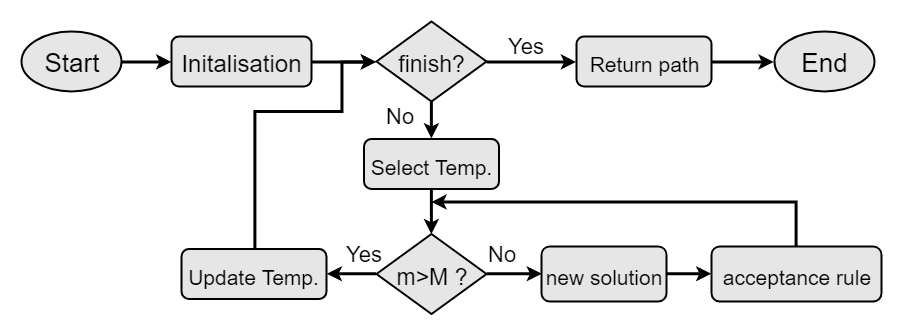
\includegraphics[width=\textwidth]{./Figures/system_implementation/LBSA.png}
  \caption{Block diagram of the Simmulated Annealing metaheuristic.}
  \label{fig:LBSA}  
\end{figure}

The majority of the SA algorithms operate on a single solution, but there are authors which 
propose a multi-agent approach \cite{multi_agent_SA}, and mention that the classic 
SA does not learn from its search history in an inteligent way, as other meta-heuristics, like the ACO, does.
Other authors focus on creating a cooling schedule which may benefit the SA algorithm, 
by enabling a more exhaustive exploration of the search space around more promosing temperatures.
An example of this is the List-Based SA algorithm proposed in \cite{list_based_SA},
which creates a cooling schedule which initially decreases faster than the traditional geometric schedule,
escaping faster from the non promising temperatures, and which than decreases slowly,
inducing a more exhaustive search around promising temperatures.  
The implementation of the Simmulated Annealing algorithm developed in this work,
follows the multi-agent and list-based chooling schedule, introduced in \cite{multi_agent_SA} and \cite{list_based_SA}.

Following the block diagram illustrated in fig \ref{fig:LBSA}, 
the algorithm receives a weight matrix describing the problem, and other relevant information,
as the duration associated to each city, and possible constraints relating the initial and final node.
The algorithm is than initialised, and some parameters must be set. This includes the initial acceptance probability $p_0$,
the maximum length of the temperature list $L_max$, the main cycle stop criteria and the markov cycle length.
The initialisation also requires the construction of an initial temperature list, which is done as follows: 

% TEMPERATURE LIST INITIALISATION
\begin{enumerate}[noitemsep,topsep=0pt,parsep=0pt,partopsep=0pt]
  \item Create an empty temperature list $L$;
  \item Create an initial solution $x$; 
  \item Create a candidate solution $y$ from $x$;
  \item If $f(y) < f(x)$, swap $x$ and $y$;
  \item Insert $t = \frac{-|f(y)-f(x)|}{p_0}$ into the temperature list;
  \item Repeat steps iii) to v) untill the temperature list reaches its maximum length;  
\end{enumerate}


The Simmulated Annealing metaheuristic is based on two cycles.
The inner cycle, often called the \textit{Markov chain},
is responsible for producing candidate solutions based on the current one.
The algorithm may accept or reject this candidate solution,
and this depends on the solutions objective function value, aswell as the current state temperature.
The Markov cycle usually runs for a fixed number of times, at each main iteration cycle.
After completing the Markov cycle, the temperature is decreased, 
and if the termination condition is not met, the Markov cycle restarts.

The process by which a candidate solution is generated is problem specific.
For the Traveling Salesman Problem, there are several suggestions in the literature,
which include, but are not limited to, 2 and 3-opt moves, insertion, reversion and swapping mechanisms.
During the development of this work, two stategies were tested.
The first follows a simple 2-opt move strategy at each markov cycle,
while the second is a greedy approach which selects the best result of the insertion, reversion and swapping functions.

At each step of the markov chain, the algorithm dictates 
that if a candidade solution is better than the current one, this solution is accepted,
and set as the current one. In its turn, if a candidate solution is worse,
it not automatically discarded, but it may be accepted.
This set of rules is refered to as the Metropolis acceptance criteria, and is defines in equation \ref{eq:metropolis_acceptance}.
The criteria sets that when confronted with a worse solution,
a random number $r: r \in [0, 1[$ is generated, and if $r$ is less than the acceptance probability, $e^{-\frac{f(y)-f(x)}{t}}$,
the candidate solution is accepted. 
This probability is such that, the lower the objective function difference,
the higher the probability of accepting the solution. On the contrary, as the state temperature decreases,
so does the acceptance probability.  

% METROPOLIS ACCEPTANCE RULE
\begin{equation}
\label{eq:metropolis_acceptance}
  p =  \left \{
  \begin{aligned}
    & 1, && \text{if}\ f(y) \leq f(x),\\
    & e^{-\frac{f(y)-f(x)}{t}},&& \text{otherwise}
  \end{aligned} \right. 
\end{equation}
  
The Simulated Annealing convergence theory suggests that this algorithm is capable of reaching the global minima, 
  










